\section{Методика использования разработанного программного средства}
\label{sec:manual}

\subsection{Системные требования}
\label{sec:manual:requirements}

Для запуска разработанного ПС требуются следующие компоненты:
\begin{itemize}
  \item операционная система на базе GNU/Linux;
  \item установленный интерпретатор языка программирования Ruby версии 2.2 или выше;
  \item установленная библиотека SDL версии 2.0.3;
  \item установленная библиотека librsvg версии 2.40.9;
  \item установленная библиотека cairo версии 1.14.2.
\end{itemize}

\subsection{Входные данные симуляции}
\label{sec:manual:input}

Входными данными для симуляции являются файл сценария симуляции и файл схемы сооружения.

\subsubsection{Файл сценария симуляции}
\label{sec:manual:input:scenario}

Файл сценария симуляции использует предметно"=ориентированный язык.
Пример сценария симуляции представлен в листинге~\ref{sec:manual:scenario_dsl_listing}.

\lstinputlisting[language=Ruby,basicstyle=\small,caption={Пример сценария симуляции}, label=sec:manual:scenario_dsl_listing, texcl=true]{sim_params_example.rb}

Все поля в данном языке объединены в секции.
Каждое поле имеет тип. Особым типом является тип <<распределение>>.
Он позволяет сгенерировать определенное значение по заданному распределению для определенных объектов в момент симуляции.
Доступными распределениями являются равномерное (uniform) и нормальное (normal).

Рассмотрим более подробно каждую секцию и поле в данном файле.

Секция scene описывает параметры сцены и содержит такие поля, как file и scale.
Поле file задает путь к файлу со схемой сооружения, который будет рассмотрен в разделе~\ref{sec:manual:input:building_scheme}.
Поле scale задает масштаб файла со схемой сооружения в метрах на пиксель.
Рекомендуется создавать файл со схемой сооружения в удобных для пользователя единицах измерения, а затем, установив параметр масштаба, задать реальные размеры сооружения.

Секция time описывает параметры времени симуляции и содержит два поля: end\_time и tick.
Поле end\_time задает время окончания симуляции в секундах. Для бесконечной симуляции можно использовать константу Float::INFINITY.
Поле tick задает длину одного шага симуляции в секундах. Рекомендуется устанавливать в поле tick достаточно маленькое значение порядка 0.1 с.

Секция spawn описывает параметры областей появления пешеходов. Ее единственным полем является поле rate, которое задает скорость появления пешеходов в людях в секунду.

Секция forces описывает социальные силы, используемые в модели.
Она имеет две подсекции: target и repulsion.
Подсекция target описывает силу притяжения пешехода к цели и имеет единственное поле "--- распределение желаемой скорости пешехода в метрах в секунду.
Подсекция repulsion описывает силу отталкивания пешехода от препятствий и также имеет единственное поле "--- распределение коэффициента отталкивания.
Рекомендуется выбирать коэффициент отталкивания около 1.0.
Данные поля имеют тип <<распределение>>, и значения по данному распределению будут сгенерированы в момент симуляции для каждого конкретного пешехода.

Секция fov описывает поле зрения пешехода.
Ее два поля "--- forward и backward "--- описывают соответственно распределения коэффициентов переднего и заднего поля зрения.
Чем больше коэффициент, тем дальше пешеход видит в данном направлении.
Значения коэффициентов примерно равны максимальному расстоянию в метрах, на котором пешеход способен различить объект.

Секция density\_map описывает параметры алгоритма определения плотностей пешеходных потоков.
Поле enabled включает либо выключает алгоритма определения плотностей пешеходных потоков.
Поля min\_threshold и max\_threshold задают соответственно минимальный и максимальный порог значений плотности.
Значения плотности ниже минимального порога не будут считаться областями скопления,
а значения равные и выше максимальному порогу будут считаться одинаково критичными областями скопления.

\subsubsection{Файл схемы сооружения}
\label{sec:manual:input:building_scheme}

Файл схемы сооружения основан на формате векторной графики SVG.
В реализованном ПС поддерживаются два основных элемента SVG "--- line и rect.

Пример схемы сооружения представлен в листинге~\ref{sec:manual:input:building_scheme:svg_listing}.

\lstinputlisting[language=XML,basicstyle=\small,caption={Пример схемы сооружения}, label=sec:manual:input:building_scheme:svg_listing]{scene.svg}

В файле допускается использование любых элементов SVG, однако для симуляции будут иметь значение только те элементы, которым проставлен атрибут x-csim-class.
Атрибут x-csim-class отвечает за тип данного элемента.  Возможные значения данного атрибута:
  wall (препятствие),
  spawn\_area (место появления людей),
  target\_area (место назначения людей "--- промежуточное или конечное).

Для элементов с классом spawn\_area и target\_area также должен быть проставлен атрибут x-csim-id.
Он задает целочисленный идентификатор пути, который связывает элементы spawn\_area и target\_area.

Для задания порядка элементов target\_area используется атрибуты x-csim-seq-no и x-csim-last.
Атрибут x-csim-seq-no задает целочисленный порядковый номер элемента target\_area в пути,
а атрибут x-csim-last устанавливает флаг окончания пути в данном элементе target\_area.

Также стоит отметить, что элементы класса wall должны быть элементами line,
а элементы классов spawn\_area и target\_area должны быть элементами rect.

\subsubsection{Запуск программного средства}
\label{sec:manual:launch}

Поддерживается запуск в двух режимах: в режиме реального времени и в режиме воспроизведения записанного ранее файла результатов симуляции.
В обоих случаях используются такие концепции операционной системы на основе GNU/Linux, как пайпы (каналы) и перенаправление стандартных потоков ввода и вывода.

Для запуска в режиме реального времени нужно выполнить следующую команду:
cat \$PATH\_TO\_SCENARIO \-|\- preprocessor/run.rb \-|\- \\ core/target/release/core \-|\- animator/animator animator/resources/person\_1.svg 1.0,
где \$PATH\_TO\_SCENARIO "--- путь к файлу со сценарием симуляции.

Снимок экрана модуля отображения результатов представлен на рисунке~\ref{sec:manual:launch:scheenshot}.

\begin{figure}[ht]
  \centering
  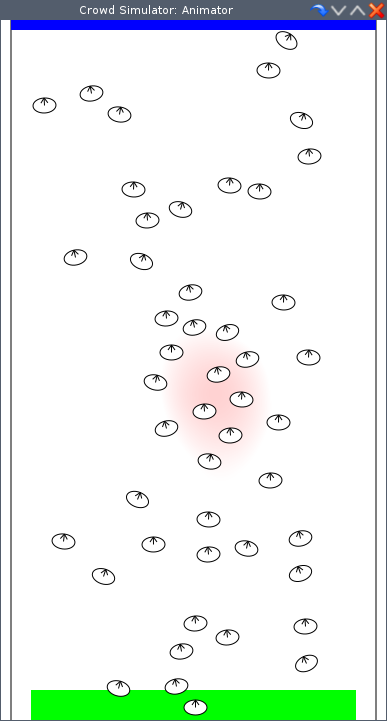
\includegraphics[scale=0.6]{screenshot}
  \caption{Снимок экрана модуля отображения результатов}
  \label{sec:manual:launch:scheenshot}
\end{figure}

Для запуска в режиме воспроизведения ранее записанного файла необходимо сначало сгенерировать файл командой
cat \$PATH\_TO\_SCENARIO \-|\- preprocessor/run.rb \-|\- core/target/release/core \->\- \$FILE\_WITH\_SIM\_RESULTS,
а затем запускать модуль отображения результатов командой \\
cat \$FILE\_WITH\_SIM\_RESULTS \-|\- animator/animator \\ animator/resources/person\_1.svg 1.0.

Также следует упомянуть возможность модуля отображения результатов использовать любую картинку в формате SVG в качестве текстуры пешехода.
Первым аргументом при запуске модуля указывается файл в формате SVG с картинкой пешехода (направление движения "--- вверх), а вторым "--- масштаб картинки в миллиметрах на пиксель.
Рекомендуется выбирать масштаб таким образом, чтобы итоговый размер пешехода был примерно равен 0.5 метра.

Пример результата работы ПС представлен на рисунке~\ref{sec:manual:launch:result_pic}.

\begin{figure}[ht]
  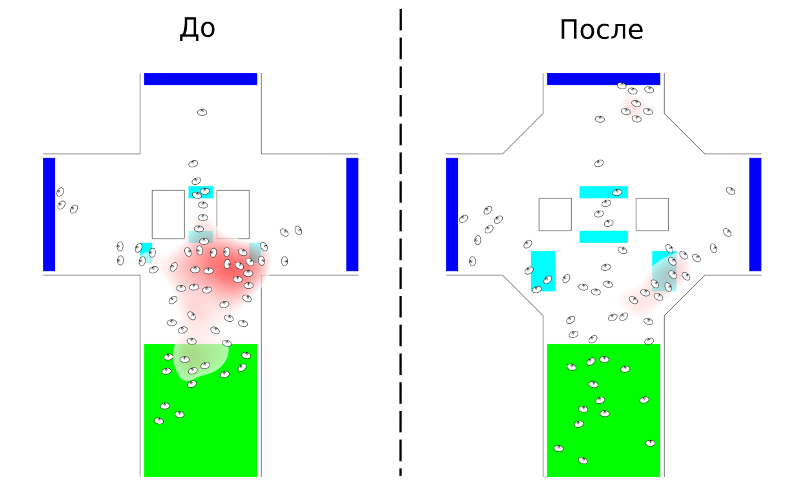
\includegraphics[width=\linewidth]{output_example}
  \caption{Пример результата работы ПС}
  \label{sec:manual:launch:result_pic}
\end{figure}
